\chapter{Concepto de anomalía}
\label{chapter:anomalia}

\section{Contextualización}

Ya hemos discutido previamente una idea intuitiva del concepto de anomalía. Un dato decimos que es anómalo cuando se distancia del resto de los datos lo suficiente como para no tener características comunes con el resto.

Este hecho puede ser por distintos motivos. Puede que la anomalía venga del hecho de que se está produciendo un evento en nuestros experimentos que no sea nada frecuente. Por ejemplo podemos estar midiendo datos meteorológicos y que en un momento dado se den una serie de fenómenos que no sea frecuente ver juntos, o incluso que no se hayan visto nunca ocurrir simultáneamente. Otra forma de tener una anomalía en nuestro conjunto de datos pudiera ser errores de medición. Por ejemplo si seguimos con este símil de los datos meteorológicos imaginemos que nuestra estación dispone de un termómetro. Este sensor se ha roto y empieza a marcar datos superiores a 100 $C^\circ$, claramente son datos muy desviados de las temperaturas normales con lo que no tendrían relación con el resto y presentaría una desviación muy importante con respecto al resto de los datos.

\section{Criterios}

Esta idea intuitiva que estamos dando de anomalía no refleja todos los posibles escenarios. Los ejemplos que estamos dando suponen una desviación muy grande de los datos normales, tanto que no se pueden comparar con el resto porque difieren mucho numéricamente. Vamos a plantear un escenario para dar una mejor forma al concepto de anomalía. Pensemos en una serie de datos muy agrupados en dos clústeres por ejemplo:

\begin{figure}[H]
	\centering
	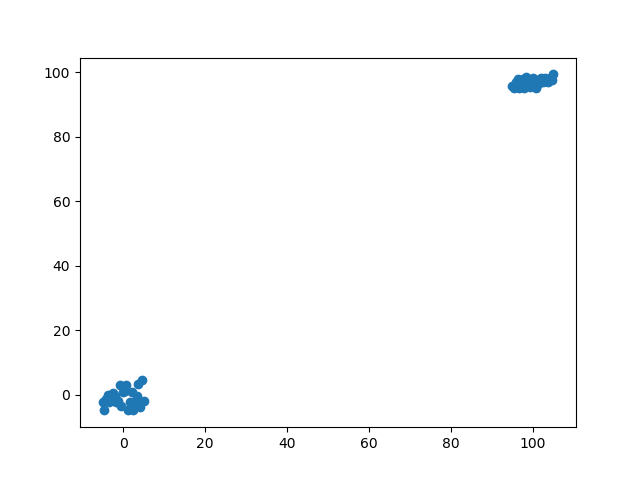
\includegraphics[scale=0.5]{imagenes/clusters}
	\label{clusters}
	\caption{Clústeres alejados}
\end{figure}

Como podemos comprobar que tenemos dos clústeres no sólo alejados entre sí, si no con los elementos muy concentrados para poner un caso extremo. Ahora no vamos a proponer un valor que se aleje de los dos clústeres, si no uno que esté a medio camino entre los dos:

\begin{figure}[H]
	\centering
	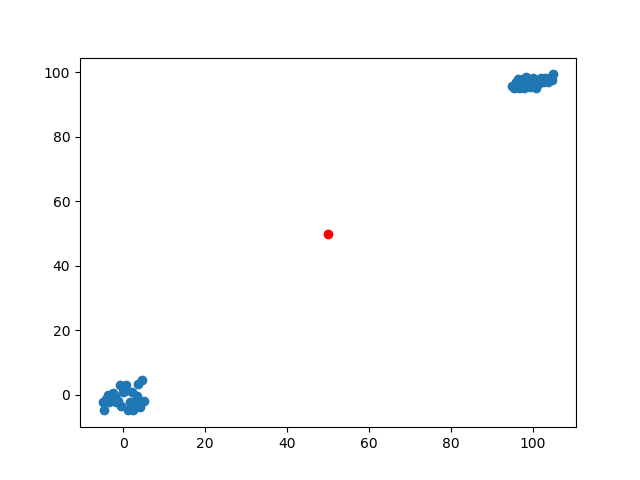
\includegraphics[scale=0.5]{imagenes/outlier_cluster}
	\label{outlier_clusters}
	\caption{Clústeres alejados con una anomalía en rojo}
\end{figure}

Si los datos del clúster de abajo a la izquierda fueran datos de temperatura con valores entorno a 0 y los de arriba a la derecha fueran de datos de temperatura entorno a 100 grados nuestro datos anómalo tendría una temperatura de unos 50 grados. Esta temperatura no se aleja radicalmente de los valores normales, es decir, no son -1000 grados ni 1000 grados. Aún así estamos describiendo una situación anómala.

No podemos dar una definición formal o que podamos decir que abarca todos los casos para definir lo que es una anomalía, aún así vamos a intentar dar dos puntos de vista: uno basado en distancias y otro en probabilidades.

El criterio más usado en la definición o detección de anomalías es el llamado ``Tukey's Fences''. Para introducirlo vamos a ver su definición en una única dimensión para luego extender el concepto. Pensemos en un conjunto de datos 1-D. Sobre sus valores podemos calcular los cuartiles $Q_1 , Q_2 $ y $Q_3$. Un valor anómalo es aquel que no cae dentro del intervalo $[Q_1 - k(Q_3 - Q_1), Q_3 + k(Q_3 - Q_1)]$ donde $k$ es una constante. El valor propuesto para $k$ por Tukey fue de $k=1.5$ aunque algunos autores más restrictivos proponen $k=3$.

Este criterio puede ser extendido al caso de mayor dimensionalidad si realizamos este mismo test sobre todos los valores de todas las características y comprobar si alguno o todos se salen del rango en función de cómo de restrictivo queremos que sea el criterio.

Esta extensión es muy vaga, por lo que se propone un criterio un poco más fijado. Imaginemos los datos agrupados por clústeres, entonces podemos fijar un centroide de dicho clúster. Sobre cada clúster podemos medir cuál es la mayor distancia dentro del clúster de los datos al centroide. Podemos extender el criterio de Tukey diciendo que un dato anómalo es aquel que se distancia más de $1.5$ veces de la mayor distancia dentro del clúster al centroide.

Esta generalización ya si abarca el ejemplo que hemos propuesto. Al estar muy apiñados los datos entorno al centroide la mayor distancia dentro del clúster es muy pequeña, de hecho en el ejemplo construido es menor que 5. Por tanto el dato $(50,50)$ está alejado más de $1.5 \cdot 5 = 7.5$ unidades del centroide y por tanto lo podemos considerar una anomalía.

\section{Qué hacer con las anomalías}

Estamos estudiando cómo podemos detectar anomalías pero una vez que las hayamos detectado en nuestros conjuntos de datos en un problema real, ¿qué debemos hacer con ellas? Este problema es algo muy general, puede que estemos seguros en nuestro caso de que las anomalías se han debido a un problema de medición porque nuestros instrumentos estaban rotos y por tanto deberíamos descartarlos. Puede que sean datos reales pero estén tan separados del resto que debamos estudiarlos de forma separada. Vamos a dar unas cuantas alternativas a lo que podemos hacer una vez que hemos detectados las anomalías dentro de nuestro conjunto de datos:

\begin{itemize}
	\item Dejarlos: puede que nuestro conjunto de datos tenga un número de datos muy elevado y por tanto aparezcan en él anomalías. Estas anomalías no deben ser eliminadas, es más debemos escoger modelos que aprendan o utilicen los datos teniendo en cuenta estas anomalías y siendo robustos ante su aparición.
	\item Exclusión: una opción es eliminar directamente las anomalías. Esto en general no está justificado y de hecho no se recomienda pues perdemos riqueza del conjunto de datos al eliminar instancias del mismo. Aún así, si decidimos eliminar los datos tenemos dos formas de hacerlo. Podemos eliminarlos directamente y prescindir de esos datos o podemos sustituirlos por datos cercanos que no sean anómalos.
	\item Estudiarlos por separado: puede que tengamos un número suficientemente elevado de las mismas y que enseñen algunos patrones o tengan explicación en nuestro ejemplo del mundo real. En este caso quizás deberíamos considerarlas y estudiarlas a parte para darles un sentido y emplear el conocimiento que les subyace.
\end{itemize}